\chapter{Похождения полковника Шукри Табета}

\begin{remark}
	Дисклеймер: эта статья представляет собой перевод с иврита интервью с Шукри Табетом, вышедшем в Журнале ВВС Израиле №130 (231) в декабре 1999 года, дополненный отрывком из книги «For Heaven's sake» Авирама Баркаи и моими комментариями. Возможны незначительные расхождения с исходнымы текстами.
	
	Мои комментарии отмечены так: (…-А.Н.). Иллюстрации взяты мной из разных источников.
\end{remark}


\textit{Интервью Табета — одно из немногих сирийских свидетельств о воздушной войне в Йом-Киппур, и одно из первых, если не первое, их подробное описание глазами сирийского пилота. И совершенно точно — первое, переведенное на русский язык}


Хоть мне и не удалось сбить ни одного израильского самолёта, но я смог уцелеть после четырёх воздушных схваток с израильскими пилотами, а это что-то значит,» — рассказывает полковник Шукри Табет, в настоящий момент — командующий палестинской вертолётной эскадрильей и бывший комэск двух боевых эскадрилий Сирийских ВВС. В Войне Йом-Киппур Шукри Табет был командующим эскадрильей МиГ-21. С большой открытостью он рассказывает о воздушных сражениях, в которых он принимал участие во время войны, описывает атмосферу в сирийских ВВС в то время и анализирует те проблемы, с которыми пришлось столкнуться сирийцам и израильтянам. «Я ничего не скрываю и не уклоняюсь от какого-либо вопроса, - говорит он, - в конце концов, это произошло уже более двадцати лет назад»

Пилоты говорят, что самое важное в воздушном бою - это умение видеть картину целиком. На учениях это просто: после приземления каждый пилот рассказывает то, что видел, а потом записи собираются в единую картину боя. В настоящих воздушных боях, на войне, полная картина недоступна никому. Потому что кое-что всегда будет упущено. Свидетельства другой стороны.

Полковник Шукри Табет, ныне командующий палестинской вертолётной эскадрильей, был командиром эскадрильи МиГ-21 в сирийских ВВС во время войны Йом-Киппур. Его версия одного из воздушных боев, которые он вел в этой войне, обеспечивает исключительную, почти уникальную возможность получить картину с другой стороны. И, в то же время, понять, насколько его видение отличается от нашего (израильского — А.Н.).

«Самая большая битва, в которой я участвовал, была в конце войны,» - говорит Табет. «Это было над Джебель-а-Шейхом за два дня до окончания войны 1973 года». «Джебель-а-Шейх» - это Хермон. Война 1973 года, конечно же, является войной Йом-Киппур.

«Бой был на средней высоте, с восемью, а может быть, с десятью самолетами «Мираж» из израильских ВВС, и я вел квартет сирийских МиГ-21, «Миражи» атаковали нас, и мы начали оборонительное маневрирование, а затем вышли из боя и вернулись обратно в Дамаск. Два пилота из моего звена получили повреждения и были вынуждены катапультироваться».

Записи ВВС Израиля о войне Йом-Киппур также упоминают этот бой. Дата: 22 октября 1973. Место: Гора Хермон.

В воздушном сражении участвовали две пары израильских самолетов Мираж (точнее, «Нэшер» — А.Н.). Подполковник (запаса) Шломо Леви, тогда заместитель командующего эскадрильей «Миражей» (113-й эскадрильи — А.Н.), вел одну из пар: «Мы еще не достигли Кирьят-Шмоны, и диспетчер уже сказал нам повернуть на восток и быть готовыми к встрече с противником. Мы сбросили баки, переключили тумблеры вооружения и включили форсаж. Мы видели перед собой сирийский квартет МиГ-21. Амос Лапидот, который был моим вторым номером, столкнулся с одной из их пар, и я остался прикрывать его. Через несколько секунд я вдруг увидел, что все небо заполнено «МиГами». Я вышел из оборонительного маневра и довернул к одному из самолетов. Я оказался в 350 метров от него. Я попытался выстрелить в него с большим упреждением, но не попал. Он маневрировал очень интенсивно, я думаю, с перегрузкой 6-7 G. Я подошел на расстоянии 150 метров от него и выпустил ещё одну очередь. На этот раз пули попали в самолет, и произошел огромный взрыв. Мне пришлось резко сбросить скорость, чтобы не врезаться в обломки».

\begin{figure}[h!tb] 
	\centering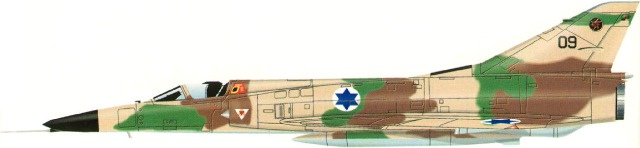
\includegraphics[scale=0.5]{History_Tabett/xSfSfyQ3-y8.jpg}
	%	\label{fig:scipion} % Unique label used for referencing the figure in-text\end{document}
	%	%\addcontentsline{toc}{figure}{Figure \ref{fig:placeholder}} % Uncomment to add the figure to the table of contents%----------------------------------------------------------------------------------------
	\caption{«Нэшер» №09 Шломо Леви. Источник: sky-high.co.il}%	CHAPTER 2
\end{figure}

«Тогда я выпустил ракету в другой самолет, примерно в 1200 метрах от меня, и я тоже сбил его, и этот пилот тоже катапультировался, и в этот момент диспетчер сообщил, что в район боя подходит множество сирийских «МиГов», и приказал мне немедленно разорвать контакт и вернуться домой. Когда мы возвращались, тот же диспетчер, но уже на другом канале наводил на цель еще двух пилотов «Миражей», Эйтана Карми и Эльдада Маяна, которые вступили в бой, когда мы уже ушли».

«Когда мы прибыли, - говорит майор (запаса) Эйтан Карми, - там уже было большое воздушное сражение. «МиГи» потеряли двоих и начали выходить из боя. То, что началось в равной борьбе, закончилось погоней. Я преследовал самолёт, который направлялся в сторону Дамаска, снижаясь ещё и ещё. Преследование продолжалось около полутора минут. У меня было мало топлива и не так много времени, я должен был уходить оттуда, потому что это была хорошо защищенная (батареями ЗРК района ПВО Дамаска — А.Н.) область, но мне всё же удалось захватить цель и выпустить ракету. Она поразила цель в полутора километрах от меня, и я видел, что сириец получил какие-то повреждения. Из-за малого остатка топлива и близости сирийских ЗРК мне нужно было возвращаться. Я не видел, катапультировался сириец, или нет. Только после возвращения я узнал, что всё же сбил его». 

\begin{figure}[h!tb] 
	\centering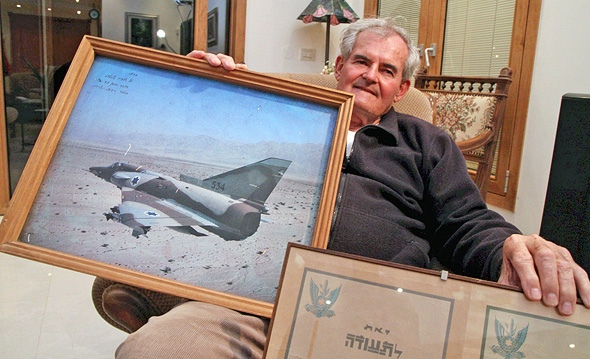
\includegraphics[scale=0.7]{History_Tabett/u5hPBTvBtpw.jpg}
	%	\label{fig:scipion} % Unique label used for referencing the figure in-text\end{document}
	%	%\addcontentsline{toc}{figure}{Figure \ref{fig:placeholder}} % Uncomment to add the figure to the table of contents%----------------------------------------------------------------------------------------
	\caption{Эйтан Карми. Фото Zohar Shachar (2015 год)}%	CHAPTER 2
\end{figure}
%\chapter*{Bibliography}
%\addcontentsline{toc}{chapter}{\textcolor{ocre}{Bibliography}} % Add a Bibliography heading to the table of contents
«Поймите, - объясняет Шукри Табет 26 лет спустя, - чтобы использовать мои ракеты, я должен был лететь с небольшой перегрузкой (пуск ракеты при перегрузке носителя более 2G был невозможен — А.Н.), а чтобы использовать пушки - оказаться на расстоянии 200-300 метров. Я должен был соблюдать ещё более жесткие условия, почти недостижимые в реальном бою.

МиГ-21 имел очень большие ограничения по ведению боя. На больших перегрузках, на самом деле, даже более 2,5 G, его оружие был практически бесполезным. Но реальные бои почти всегда проходили на больших перегрузках — что нам было делать? Мы летали на этом самолете, и все мы были очень недовольны, потому что мы знали, что у нас были плохие радары и ракеты (радар «Миража» по мнению израильтян был также столь плох, что они заменяли его на балласт — А.Н.). Мы были словно два разных человека — у одного оружие времён Второй Мировой, а у другого — самое современное». 
%------------------------------------------------


\begin{figure}[h!tb] 
	\centering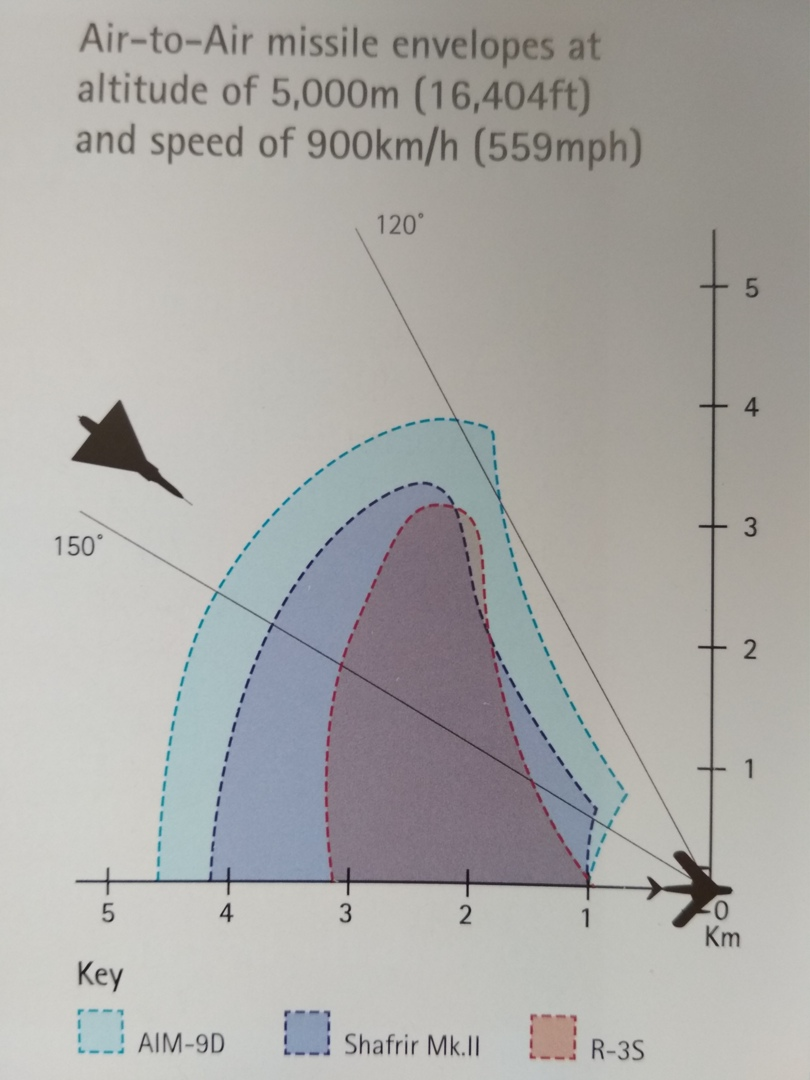
\includegraphics[scale=0.4]{History_Tabett/7v_taieZfE0.jpg}
	%	\label{fig:scipion} % Unique label used for referencing the figure in-text\end{document}
	%	%\addcontentsline{toc}{figure}{Figure \ref{fig:placeholder}} % Uncomment to add the figure to the table of contents%----------------------------------------------------------------------------------------
	\caption{Сравнение областей пуска ракет сирийцев и израильтян, фото из книги Arab Migs (vol.5 October War 1973: part 1) Тома Купера. }%	CHAPTER 2
\end{figure}

\section{Летный курс в Сирии и СССР}

Во время войны Йом-Киппур полковник Шукри Табет служил в сирийских военно-воздушных силах, но первоначально он был палестинцем, который иммигрировал в Сирию. Шесть лет назад, сразу после подписания Ословских соглашений, он вернулся в Газу и был назначен командующим вертолетной эскадрильей. Он родился в 1946 году в Беэр-Шеве, седьмом ребенке семьи Табет. У него три брата и три сестры. Когда ему было один год, его семья переехала в Газу. Он окончил среднюю школу в Газе, со специализацией в физике. Он всегда любил самолеты и мечтал стать летчиком, он говорит о себе:

«В 1964 году, когда я окончил среднюю школу, я переехал в Дамаск, где вся моя семья осталась в лагере беженцев в Джабалье, а через год меня приняли в Колледж Дамаска и я начал изучать право. Я увидел объявление, призывающее добровольцев на сирийский воздушный курс, я увидел возможность и решил воспользоваться этим, всё, что я хотел, было стать офицером в армии, а в Сирии, как и везде, наиболее престижно было стать лётчиком».

В 1967 году Шукри Табет начал курс. «Первый год курса был у основания Алеппо, на севере Сирии,» - говорит он. «Это были теоретические исследования и полет на «Бурундуках» (легкий учебный самолет из Канады) и L-39 (чешский учебный самолет). Летчики-истребители Сирийских ВВС второй год обучаются в Краснодаре, на Украине (так в оригинальном интервью— А.Н.), где я летал на МиГ-21. Я был единственным палестинцем на сирийском лётном курсе, но оба инструктора и курсанты обращались ко мне так же, как и ко всем остальным».

В 1969 году Табет завершил лётный курс в СССР и вернулся в Сирию в качестве молодого лейтенанта, пилота МиГ-21. Там, под Дамаском, он продолжил курсы и тренировался с инструкторами из СССР и Сирии. В течение года он жил один в Дамаске, пока не женился на девушке, с которой он встретился в Газе. «Я написал моей семье в Газе, что хочу жениться на ней, они согласились, и ее отправили в Дамаск».

В войне Йом-Киппур или войне 1973 года, как он ее называет, он находился на авиабазе Сигаль под Дамаском и командовал эскадрильей МиГ-21 (эскадрильей №11 - А.Н.). «В течение первых пяти дней мы занимались разведкой и прикрытием сирийских танков, но с шестого дня я участвовал в четырех воздушных боях против израильских летчиков, которые летали на «Фантомах» и «Миражах». 

\begin{figure}[h!tb] 
	\centering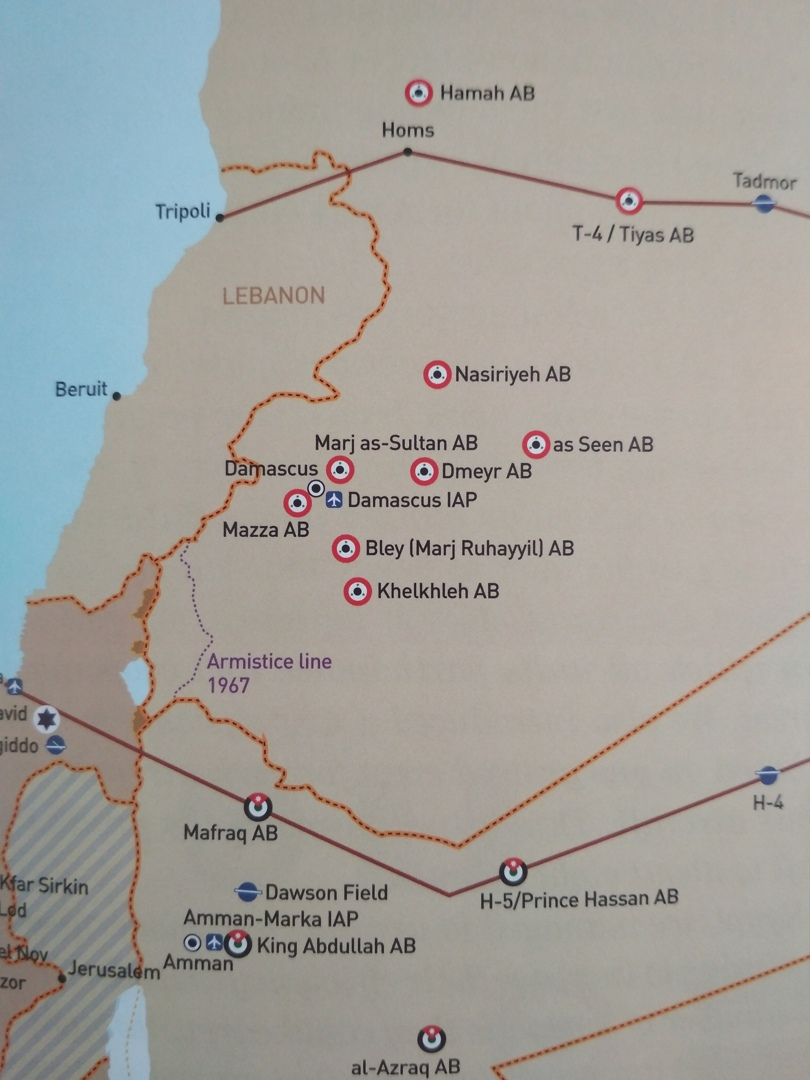
\includegraphics[scale=0.4]{History_Tabett/gKKUZb6lodU.jpg}
	%	\label{fig:scipion} % Unique label used for referencing the figure in-text\end{document}
	%	%\addcontentsline{toc}{figure}{Figure \ref{fig:placeholder}} % Uncomment to add the figure to the table of contents%----------------------------------------------------------------------------------------
	\caption{Сирийские авиабазы, фото из книги Arab Migs (vol.5 October War 1973: part 1) Тома Купера. Хулхуле находится несколько южнее Дамаска.}%	CHAPTER 2
\end{figure}

«Битва в районе Хермона была самой большой, в которой мне довелось участвовать, но были и другие события, например, в середине войны я участвовал в бою над авиабазой Хулуле недалеко от Дамаска. Я был в патрулировании на большой высоте и увидел четыре израильских «Фантома», летящих на небольшой высоте, готовых атаковать взлётно-посадочную полосу. Я понял, что они атакую через несколько секунд, и я выпустил ракету в сторону ведущего самолёта, чтобы привлечь их внимание, но, к моему удивлению, они всё равно продолжили атаку. К моему удивлению, потом они были готовы и к воздушному бою».

И снова вернёмся к описанию того боя в ВВС Израиля, которые полностью совпадают со словами сирийского лётчика. «12 октября, в 6:50, четвёрка «Фантомов» атаковала сирийскую авиабазу Хулхуле», - говорится в докладе. «Пока они все еще были в воздухе, другие экипажи сообщали о появлении «МиГов» в воздухе. Во время удара был также зафиксирован плотный зенитный огонь».

«Это была обычная рутина, - рассказывает полковник (в отставке) Амнон Гурион, который возглавлял атаку. - Район авиабазы Хулхуле был сложным. Там было много зениток, и результаты ударов по ним были хуже, чем мы привыкли видеть. Я думаю, сирийские средства РЭБ тоже доставили проблем. Я помню, что в этом рейде был очень серьезный зенитный огонь, артиллерии и ракет, мы просто были поглощены морем взрывов вокруг, но «МиГов» близко мы не видели». (на самом деле, здесь произошла некоторая путаница. Звено Амнона Гуриона атаковала авиабазу Хулхуле, а бой с «МиГами» был несколько севернее, над аэродромом «Дамаск-международный», об этом ниже - А.Н. Также отметим, что это был уже четвёртый налёт на эту авиабазу в 73-м году). 

\section{Против солнца}

Табет улыбается, открыто говорит. «Мне все равно, - говорит он, - я ничего не скрываю и не избегаю никаких вопросов».

\textit{После всех боёв, в которых вы участвовали, что вы думаете об израильских летчиках? }

«Еще до войны было несколько воздушных боев, в которых я не участвовал, но я слышал о них всех, и я говорю вам, что израильские летчики показали себя лучше до войны, чем во время войны».

\textit{Почему?}

«Потому что израильские военно-воздушные силы были вынуждены воевать по совсем другим правилам. Раньше израильтяне все время диктовали условия, и на этот раз они (арабы - А.Н.) подготовились, и подготовились очень хорошо. Например, до 1973 года, израильтяне всегда планировали воздушные бои так, чтобы солнце светило в глаза египетским пилотам, а в 1973 году было наоборот.

Израильтяне всегда провоцировали нас на атаку, выманивая наши самолёты своими, которые было хорошо видно на египетских и сирийских радарах. А когда наши «МиГи» поднимались, чтобы перехватить их, то на малой высоте их ожидали невидимые для РЛС израильские самолеты, и когда сирийские или египетские самолеты взлетали, израильтяне атаковали их снизу вверх — в идеальной позиции для пуска ракет. Таким образом, они и достигали хороших результатов. Но все это было до 1973 года. Израильтяне владели инициативой, они решали, где и когда будет сражение. Везде были ловушки, засады. В 1973 году не было засад. Бои были лицом к лицу.

Израильским пилотам повезло, им повезло иметь хорошее оружие и хорошие радары».

\textit{Разница, на ваш взгляд, в технике?}

«Да, сирийские летчики очень храбры, очень талантливы и хорошо обучены, но в 1973 году израильтяне были лучше вооружены. Я должен признать, что я понятия не имею, каков ваш уровень сейчас, и последний раз, когда я летал на истребителе, это было более 10 лет назад, это был МиГ-21 в Йемене, и сегодня воздушный бой изменился, и теперь больше полагаются на технику. Раньше это было не так, и сегодня наше оружие тоже стало другим. Например, эти новые ракеты, «выстрелил и забыл».

\textit{Какова была атмосфера сирийских ВВС во время войны?}

«В первые пять-шесть дней войны боевой дух сирийских ВВС был высоким, а затем, когда вы начали атаковать цели в Сирии, Дамаске, сирийская армия отступала с Голан, то и настроение менялось. Хотя ни один из моих близких друзей не был убит на войне, в моей эскадрилье были погибшие».

\textit{Вы сами сбивали израильские военные самолеты?}

«Нет, мне не удалось сбить израильский самолет, но остаться в живых после четырех битв с вашими ВВС что-то значит, значит, что я хорошо летал».

Вертолеты Раиса ("президента" - А.Н.)

После войны Йом Киппур, Шукри Табет переучился на МиГ-23. В течение следующих четырех лет он служил летчиком, а затем командиром эскадрильи в эскадрилье МиГ-23 на базе около Дамаска.

«Я оставался в сирийских военно-воздушных силах до конца 1978 года, когда между лоялистами Сирии и палестинцами в Ливане вспыхнула борьба, у нас было очень мало палестинских офицеров в сирийских военно-воздушных силах, шесть, максимум восемь, и, насколько я знаю, я был единственным пилотом. Я считал себя сирийцем на сто процентов, но когда сирийские ВВС сражались против палестинцев в Сирии и Ливане, все изменилось, и я не мог больше участвовать в этой войне, поэтому я ушел. Это была война в Ливане, и я не мог оставаться в Сирии. Мне очень жаль, что сирийская армия напала на палестинцев тогда».

В конце 1970-х годов Табет, который был объявлен дезертиром из сирийской армии, присоединился к Force 14, ВВС Яссира Арафата, с двумя целями: сформировать ядро для ВВС в создаваемом палестинском государстве, и оказать содействие в транспортировке членов организации на Ближнем Востоке, для которого молодые палестинцы были отправлены в арабские страны для прохождения обучения, а затем были отправлены в штаб-квартиру в Тунисе.

«В течение года я был инструктором в Алжире, затем четыре года в Ливии, на МиГ-23, и когда я закончил свою работу в Ливии, я тренировал на МиГ-21 в Йемене десять лет». В какой-то момент он был назначен командующим Force 14. Он не хотел рассказывать об этом периоде. «Все было — обучение, полёты и лекции».

Табет впервые встретился с Ясиром Арафатом в Бейруте в 1978 году. Когда были подписаны соглашения в Осло, Арафат позвонил ему и предложил ему присоединиться к вертолетной эскадрилье Палестинской автономии, расположенной в Газе. Конечно, Тебет посчитал это большой честью. По сей день, смотря на фото с его тщательно отглаженной оливковой формой, знаками отличия полковника и «крыльями» лётчика, с огромным пистолетом, висящим в кобуре на поясе справа, вы можете видеть, как его лицо сияет от счастья. 

\begin{figure}[h!tb] 
	\centering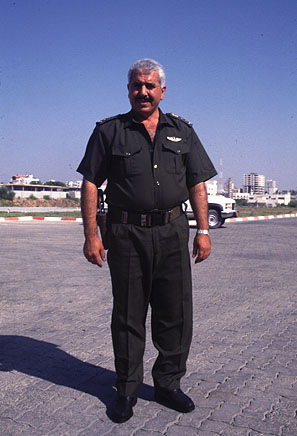
\includegraphics[scale=0.8]{History_Tabett/uwRpBNzkdFk.jpg}
	%	\label{fig:scipion} % Unique label used for referencing the figure in-text\end{document}
	%	%\addcontentsline{toc}{figure}{Figure \ref{fig:placeholder}} % Uncomment to add the figure to the table of contents%----------------------------------------------------------------------------------------
	\caption{Полковник Табет, 1999 год. Фото из Журнала ВВС Израиля}%	CHAPTER 2
\end{figure}

Вертолетная эскадрилья Палестинской администрации была расположена в западной части Газы, прямо на пляже, в нескольких минутах ходьбы от дома Арафата. В состав эскадры входили три Ми-17, российских транспортных вертолета. Красивые , компактные, полированные, окрашенные в белый цвет с зеленой полосой в центре. Внутри вертолеты еще более впечатляют. Очень просторные, с элегантными креслами и новой обивкой. Совершенно отличаются от израильских вертолетов, с вертикальными жесткими армейскими стульями и масляными пятнами вокруг отверстий в потолке.

\begin{figure}[h!tb] 
	\centering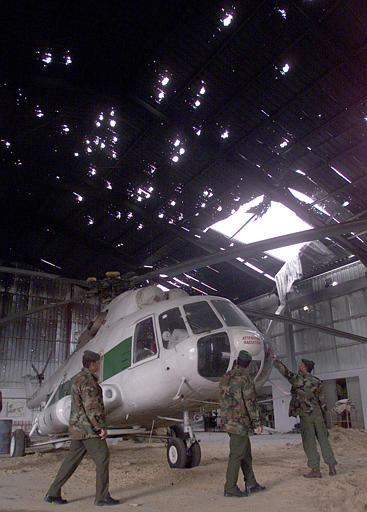
\includegraphics[scale=0.8]{History_Tabett/ryAlPiWH3Xc.jpg}
	%	\label{fig:scipion} % Unique label used for referencing the figure in-text\end{document}
	%	%\addcontentsline{toc}{figure}{Figure \ref{fig:placeholder}} % Uncomment to add the figure to the table of contents%----------------------------------------------------------------------------------------
	\caption{Один из вертолётов «Подразделения 14» в Газе, 2001 год. Ангар были уничтожен израильской ракетой.}%	CHAPTER 2
\end{figure}

Рядом с ангаром стоят два вертолета. Третий вертолет — в России на ремонте. Они предназначены только для одной цели — перевозить Арафата, и постоянно находятся на линии Газа-Газа-Газа, а иногда и Газа-Каир. «Когда не используются три вертолета, у меня есть время для проведения учебных полётов для молодых пилотов,» - объясняет Табет. «Теперь у меня их всего два, а два вертолета - это минимальное количество, так что сейчас они не тренируются».

Сам Табет никогда не летал на вертолете. Он, как уже упоминалось, истребитель. Но он отвечает за вертолеты, полеты и подготовку палестинских летчиков, местных жителей. Между тем, для эксплуатации вертолетов были специально привезены два опытных российских летчика-испытателя. «Тем не менее, - говорит Табет, - это раис, это не просто пассажир».

Сегодня Шукри Табет живет со своей женой и тремя дочерьми в Газе. У него есть брат и сестра в Аммане, брат и сестра в Газе, брат в Ливии и сестра в Рамалле. «Все мои дочери родились в Дамаске, все они путешествовали со мной на протяжении многих лет, все они закончили университет в Газе или все еще учатся, одна работает в области медицинских исследований, вторая изучает английскую литературу, третья - физику. Моему сыну Ахмеду — год».

\textit{Хочешь, чтобы он был пилотом?}

«Ни в коем случае! Вместе со мной курс закончили двадцать шесть человек, шесть лет спустя, девять из них уже не было в живых, а сегодня осталось только четверо... Быть боевым пилотом - опасная профессия... Лично мне это очень нравилось, но я бы не хотел этого для людей, которых я люблю. Но если бы я мог снова начать свою жизнь, я бы снова решил стать летчиком-истребителем».

В дополнение к своей роли командира палестинской эскадрильи вертолетов Шукри Табет является членом израильско-палестинского совместного аэрокосмического комитета. «Благодаря долгим часам переговоров и обсуждений я нашел настоящих друзей в ваших ВВС,» - радостно говорит он.

Табет говорит о подполковнике Алоне, который до недавнего времени занимал пост главы международной координации в IAF, а Алон, пилот F-16, ушел в отставку из IDF несколько недель назад. В честь его отставки полковник Табет пригласил подполковника Алона на праздничный обед.

‌«Мы работали вместе четыре года без соглашений и без протокола, и мы передали их очень позитивно, без сучка и задоринки, без кризисов, как будто все было подписано,» - сказал Табет. «Как у боевого лётчика, у меня была возможность в прошлом стрелять в вас, и у меня, конечно же, было такое же чувство: если бы я встретил израильтянина тогда, в воздушном сражении, я бы думал только об одном — как его убить. Сейчас… сейчас мы все должны жить в мире, другого пути нет». 

\section{На этом интервью заканчивается.}

Как я писал выше, в комментариях, в статье есть некоторая путаница в том, что касается боя 12 октября. Фактически, он проходил южнее Дамаска, когда четвёрка «Фантомов» 201-й эскадрильи, атаковавшая аэропорт Дамаска уходила от цели в сторону Голан. В это же время, другое звено бомбило Хулхуле — неудивительно, что сирийский комэск их перепутал!

Что касается боя с МиГ-ами, он тоже был и достаточно подробно описан в книге «От имени Неба» (For Heaven's sake) Авирама Баркаи. Мне кажется, стоит привести этот отрывок полностью — есть предположение, что в ней достаточно подробно описан тот самый бой, о котором упоминает сирийский комэск. Да и вообще отрывок достаточно показательный:

\begin{textcitation}
	«Регев! На инструктаж!» - орёт громкоговоритель, как только Гиль Регев переступил порог здания Эскадрильи, после перегона самолёта из Шарм - эль Шейха – завершающей стадии его ночных приключений. 
	
	«Сирийцы хорошо восприняли уроки Шестидневной Войны» - говорят им на инструктаже перед новым заданием – «Подвергшиеся недавним атакам аэродромы уже вернулись в действие. Нам надо повторно разбомбить аэродромы Дамаск-Международный и Хулхуле». 
	
	Гиль Регев невольно содрогается – "Дамаск, это там сейчас электрошоком пытают Шани-боя и Асаэля. А у меня штурманом поставили молодого Шмуэли – это тебе не хладнокровный Бар-Ам. И это не спокойный Шарм Эль Шейх". 
	
	В 06:10 четвёрка Фантомов, цель которых аэродром Дамаск-Международный, взлетает и образцово собирается в звено, равняясь на ведущего, капитана (запаса) Ади Бная. 
	
	Позади долины Ливана, впереди последний отрезок маршрута на Дамаск. Над городом и его окрестностями лежит тёмная пелена.
	«Интересное сочетание» - думает ведущий, Ади Бная – «Пары влаги вместе с дымом и пеплом от горящих нефтехранилищ, которые мы бомбили вчера».
	«Первый! Внимание!» - сообщает второй номер, Итамар Барнеа, летящий вслед за Бная – «Четвёрка МИГ-ов высоко над нами!». 
	
	«Вижу» - отвечает Ади Бная – «Продолжаем!» 
	
	И командует, своим спокойным голосом, как будто на учениях по бомбометанию – «Опуститься под полосу дыма!» 
	
	«Отлично!» - думает в ведущем самолёте Ади Бная – «Задание было атаковать и уничтожить. Мы это сделали - атаковали и уничтожили. Сейчас лишь бы небо оставалось чистым – у нас нет топлива для воздушного боя».
	Домой! Он делает широкий разворот, чтобы собрать звено, считает самолёты. Одним больше! «Четвёртый, у тебя МИГ на 12 часов!» - сообщает он Гили Регеву.
	
	«Гиль! Крутой вираж! МИГ!» - орёт штурман. 
	
	Гиль закладывает крутой вираж, но самолёт ведёт себя как ленивый бык, а не резвый скакун. 
	
	«Гиль! Вираж!!» 
	
	Гиль закладывает другой крутой вираж, и думает «Чёрт! Так ведь этот МИГ ещё его и поймает!» 
	
	«Ойш!» - срывается у него, когда он замечает, что забыл сбросить бидоны перед началом крутых манёвров. Нажимает кнопку «PANIC» и улыбается про себя, чувствуя, как его Фантом резвеет. 
	
	Но МИГ всё ещё за ними. «Погоди, придурок!» - думает Гиль – «Дай набрать скорость! И тогда посмотрим!». Гиль выполняет крутой манёвр, как учил его Шани-бой, и под солнцезащитном щитком лётной каски улыбка начинает расплываться на его лице. МИГ пролетает мимо, Гиль резвым разворотом заходит ему в хвост, выпускает ракету воздух-воздух, которая догоняет МИГ и вколачивает его в землю. 
	
	Ади Бная интересуется, своим спокойным голосом - «Четвёртый! Ты где?».
	Но именно в этот момент другой МИГ заходит на Фантом Гиля Регева и отрывает по нему пушечный огонь. Шмуэли, штурман Гиля Регева, видит пламя пушечных выстрелов, загипнотизировано смотрит на белую каску Сирийского лётчика, который хочет их убить, и думает, что ещё чуть – чуть, и он умрёт.
	«Вираж, сукин сын, вираж!!» - орёт Шмуэли, повторяя знаменитый боевой клич Йосариана из известной книги «Уловка 22». 
	
	«Четвёртый! Ты где?» 
	
	Гиль Регев маневрирует, уходит вниз, чтобы добрать скорость, от перегрузок кислородная маска сползает вниз, и он хрипя отвечает ведущему звена – «Четвёртый в замесе с МИГ-ами!». 
	
	Но Бная, не понимая слов в хрипе Гиля, опять повторяет «Четвёртый! Ты где?»
	Гиль знает, что он всё ещё над Дамаском, и что отсюда надо уносить ноги, а для этого надо сделать ещё парочку крутых манёвров и набрать скорость при помощи форсажной камеры, но для этого у него нет топлива.
	
	Бум! Что то ударило в самолёт?
	«Четвёртый! Ты где?»
	«Четвёртый не может вас догнать!» - поправив маску рапортует Гиль - «В замесе с МИГ-ами!» 
	
	«Надо спасать четвёртого!» - думает третий номер, майор Эли Зоар, разворачивается и на полном форсаже мчится назад, к Дамаску. Находит Гиля, увёртывающегося от МИГ-а, заходит на того, целится, нажимает на кнопку запуска ракет воздух-воздух. Ничего не происходит! 
	
	«Чёрт! Почему ракеты не работают!?» - вопрошает-протестует Зоар, хрипя от перегрузок манёвра. 
	
	А «Носорог», который сам борется с перегрузкой и недостатком кислорода, результатом сползающей от тех же перегрузок потной кислородной маски, уже позабыл дискуссию после взлёта про переключатели ракет воздух-воздух, и хрипит в ответ «Не знаю». 
	
	В конце концов, МИГ замечает, что за ним гонится второй Фантом, и оставляет Гиля Регева в покое. Все собираются вместе и продолжают домой. Кто то докладывает Гилю, что у него в крыле дыра размером с ведро – «бум», который они почувствовали в схватке с МИГ-ом был реальным.
	«Дотяни, дружище! Дотяни» - умоляет Гиль свой Фантом. 
	
	В 06:50 пока четвёрка Ади Бная воюет с МИГ-ами над Дамаском, другая четвёрка Эскадрильи, ведомая Амноном Гурионом разбивает на куски ВПП аэродрома Хулхуле. Для Фантомов Эскадрильи это четвёртый визит на этот аэродром. Для Сирийцев доказательство, что имеют дело с ВВС и с эскадрильей бульдогов, которые вцепившись, не отпускают свою жертву, пока не завершат начатое, или им не дадут другую команду. 
\end{textcitation}

%Источники \cite{tabet_article,barkai,segev,misnikov,kuper_nikole}.
Источники:
\begin{itemize}
	\item "Журнал ВВС Израиля" №130 (231) декабрь 1999 года, статья Лион Шлейн «Полковник Табет».

\item «От имени Неба», Авирам Баркаи.

\item Сайты Амира Сегева (sky-high.co.il), Авиноама Мисникова (Мерхав Авири), skywar.ru.

\item Книги Тома Купера и Дэвида Николле.
\end{itemize}

Ссылка на оригинал \url{https://vk.com/wall-162479647_36561}

К оглавлению на странице \pageref{tablecont}